\section{Interpretation}
\label{sec:Interpretation}

This section explains how to interpret a trace view once it has been adjusted as 
described in the previous section.

\begin{itemize}
 \item The trace view has on its horizontal axis the execution time and on the vertical 
       axis one line for the master at the top, and below it, one line for each of the workers.
 \item In a line, the light blue color is associated with an idle state, i.e. there is no event at that time.
 \item Whenever an event starts or ends a flag is shown.
 \item In the middle of an event, the line shows a different color. Colors are assigned depending on the event type.
 \item The info panel contains the legend of the assigned colors to each event type.
\end{itemize}

\begin{figure}[ht!]
  \centering
    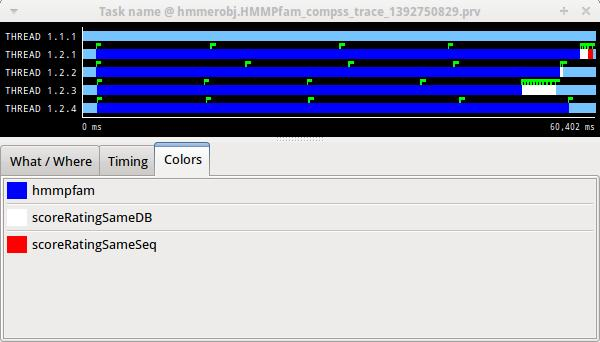
\includegraphics[width=\textwidth]{./Sections/4_Interpretation/Figures/7.jpeg}
    \caption{Trace interpretation}
\end{figure}